\documentclass{article}
\begin{document}
\subsection{Running example on PC side via BLE}
The sequence of actions required for interfacing via BLE includes the steps below:
\begin{enumerate}
	\item Go to the examples folder in file explorer.
	\item Open the common.c file in the selected example folder in your IDE.
	\item Change COINES\_COMM\_INTF\_USB  to COINES\_COMM\_INTF\_BLE.
	\item Connect the Application board to another power source and keep it within the BLE range.
	\item Now follow the same steps from 3 - 6 in the above section.
	\begin{figure}[H]
		\begin{center}
			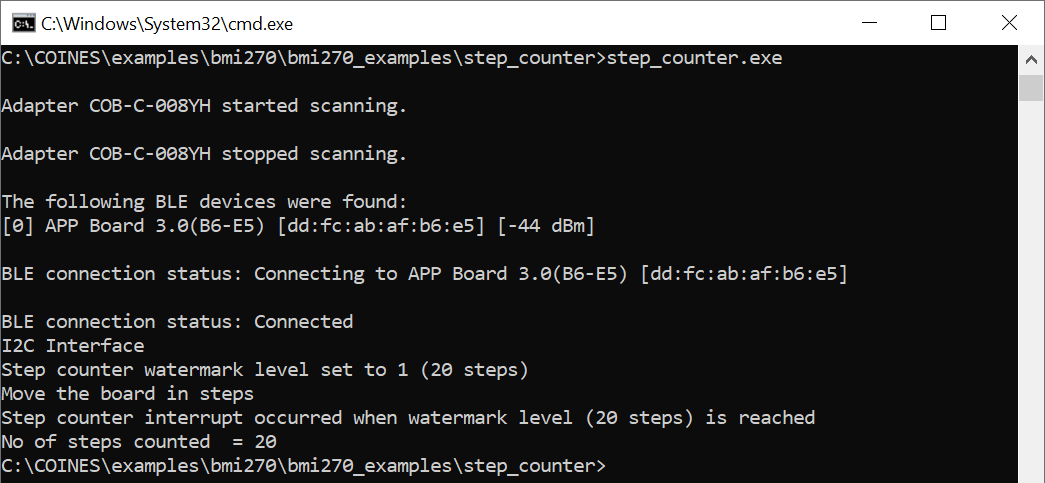
\includegraphics[width=0.9\textwidth]{coinesAPI_images/Pc_example_ble_output.png}
		\end{center}
	\end{figure}
\end{enumerate}
\newpage

\end{document}